\hypertarget{organizational-diversity}{%
\section{Organizational Diversity}\label{organizational-diversity}}

Question: What is the organizational diversity of contributions?

\hypertarget{description}{%
\subsection{Description}\label{description}}

Organizational diversity expresses how many different organizations are
involved in a project and how involved different organizations are
compared to one another.

\hypertarget{objectives}{%
\subsection{Objectives}\label{objectives}}

\begin{itemize}
\tightlist
\item
  Get a list of organizations contributing to a project.
\item
  See the percentage of contributions from each organization within a
  defined period of time.
\item
  See the change of composition of organizations within a defined period
  of time.
\item
  Get a list of people that are associated with each organization.
\end{itemize}

\hypertarget{implementation}{%
\subsection{Implementation}\label{implementation}}

\begin{itemize}
\tightlist
\item
  Collect data from data sources where contributions occur.
\item
  Identify contributor affiliations to get a good estimate of which
  organizations they belong to.
\item
  Correlate information about contributions, assigning each to
  appropriate organization.
\item
  Depending on the needs of the project, you may want to consider such
  issues as how to handle multiple email addresses, affiliation changes
  over time, or contractor vs. employee.
\end{itemize}

\hypertarget{tools-providing-the-metric}{%
\subsubsection{Tools Providing the
Metric}\label{tools-providing-the-metric}}

\begin{itemize}
\item
  \href{https://chaoss.github.io/grimoirelab}{GrimoireLab} supports
  organizational diversity metrics out of the box. The
  \href{https://github.com/chaoss/grimoirelab-sortinghat}{GrimoireLab
  SortingHat} manages identities. The
  \href{https://github.com/chaoss/grimoirelab-hatstall}{GrimoireLab
  Hatstall} user interface allows correcting organizational affiliation
  of people and even recording affiliation changes.

  \begin{itemize}
  \item
    View an example visualization on the
    \href{https://chaoss.biterg.io/app/kibana\#/dashboard/Community-Structure-by-Organization}{CHAOSS
    instance of Bitergia Analytics}.
  \item
    Download and import a ready-to-go dashboard containing examples for
    this metric visualization from the
    \href{https://chaoss.github.io/grimoirelab-sigils/panels/community-structure-by-organization/}{GrimoireLab
    Sigils panel collection}.
  \item
    Add a sample visualization to any GrimoreLab Kibiter dashboard
    following these instructions:

    \begin{itemize}
    \tightlist
    \item
      Create a new Pie chart

      \begin{itemize}
      \tightlist
      \item
        Select the \texttt{all\_onion} index
      \item
        Metrics Slice Size: \texttt{Sum} Aggregation,
        \texttt{contributions} Field, \texttt{Contributions} Custom
        Label
      \item
        Buckets Split Slices: \texttt{Terms} Aggregation,
        \texttt{author\_or\_name} Field, \texttt{metric:\ Contributions}
        Order By, \texttt{Descending} Order, \texttt{500} Size,
        \texttt{Organization} Custom Label
      \end{itemize}
    \item
      Example Screenshot
    \end{itemize}

    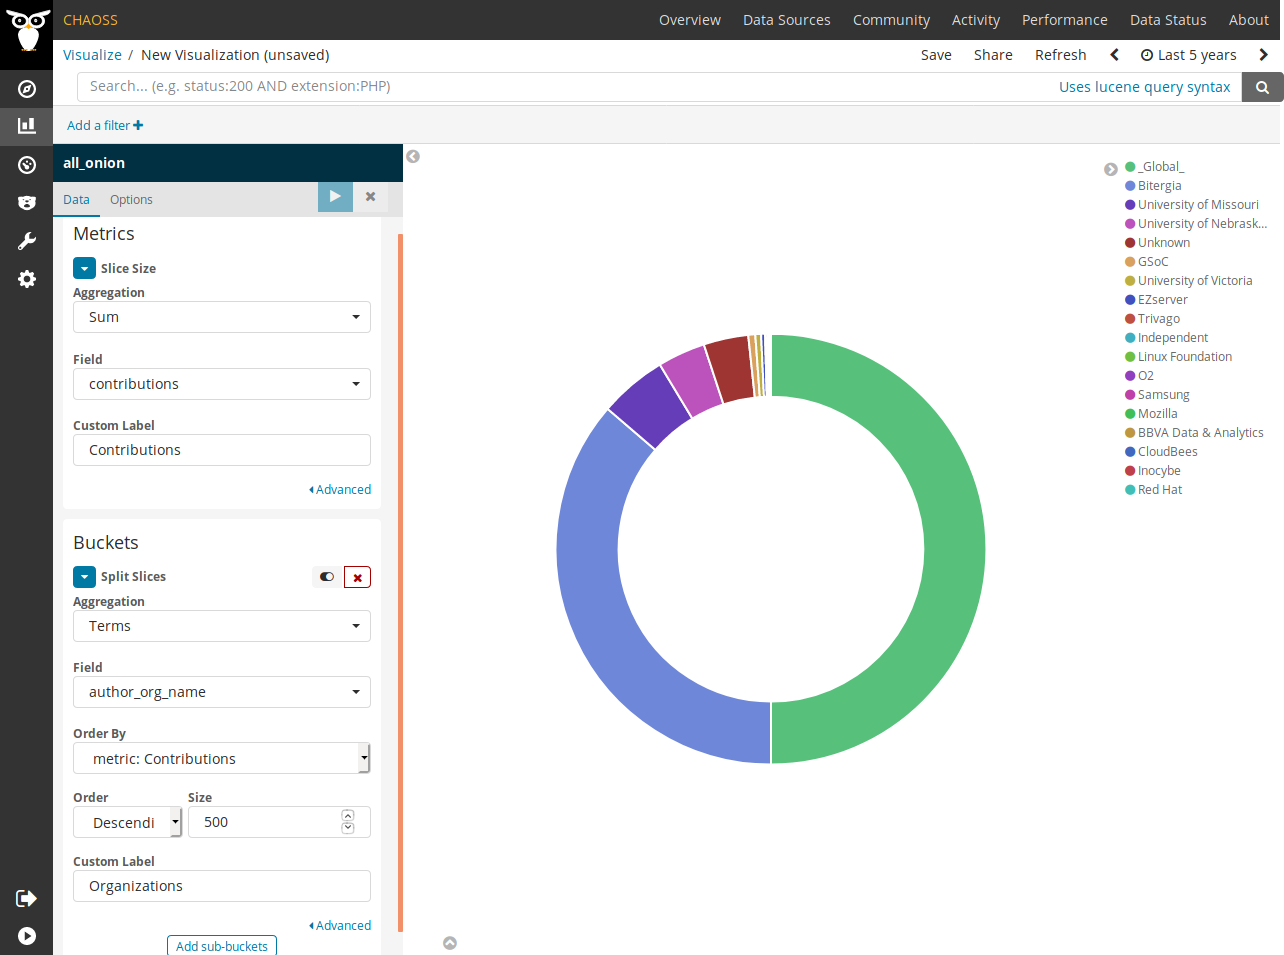
\includegraphics{images/organizational-diversity_piechart.png}
  \end{itemize}
\item
  \href{https://lfanalytics.io}{LF Analytics} provides organization
  diversity metrics in the primary view for commits, issues filed, and
  communication channels (current support for Slack and groups.io)
\end{itemize}

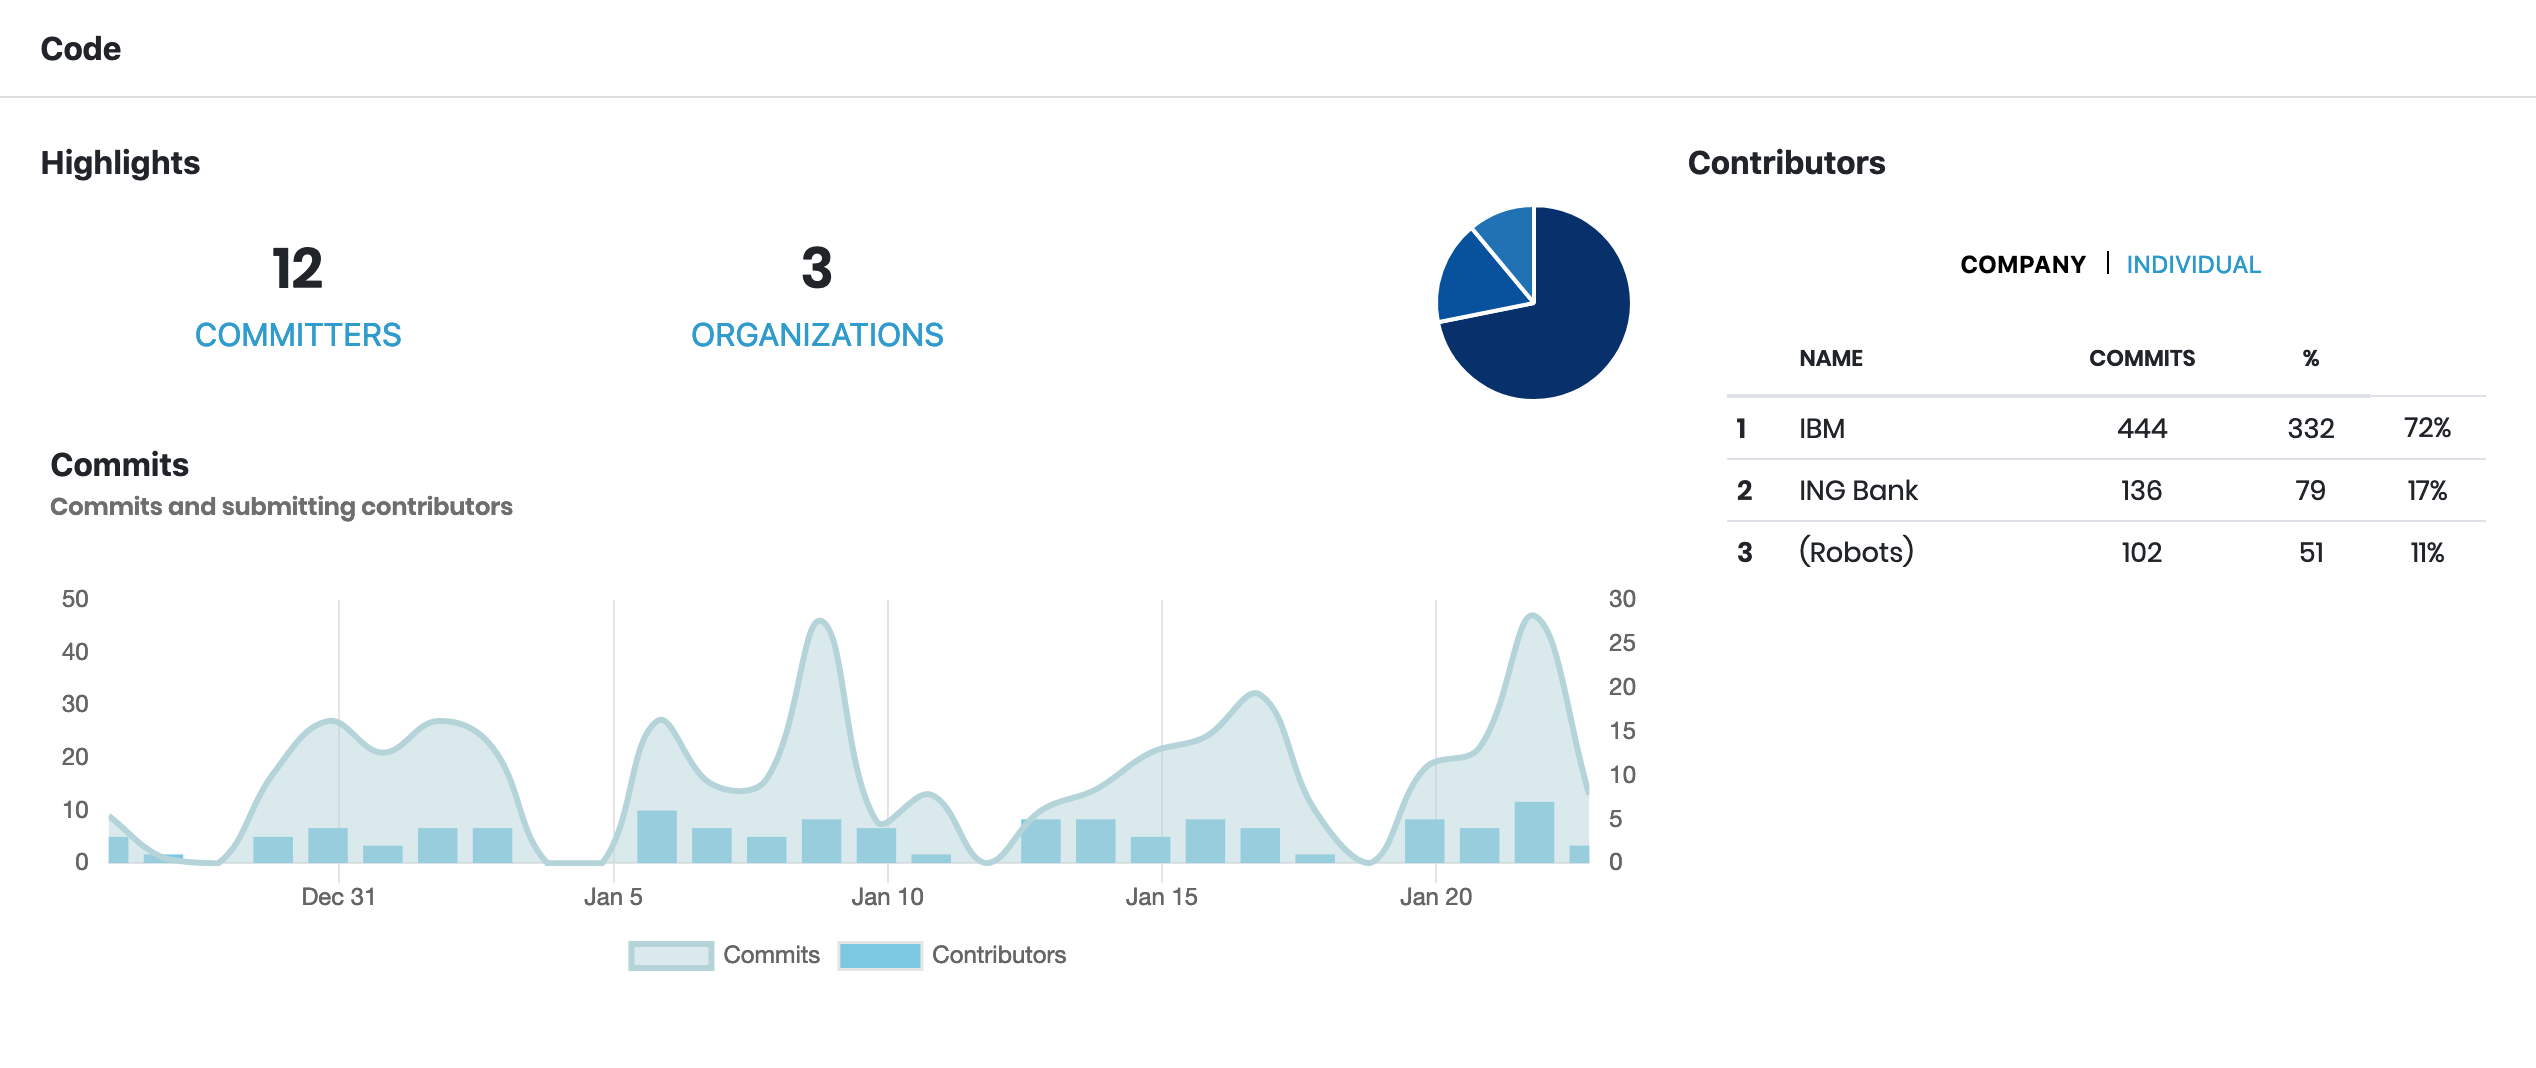
\includegraphics{images/organizational-diversity_lfanalytics-orgdiversity.png}

\hypertarget{data-collection-strategies}{%
\subsubsection{Data Collection
Strategies}\label{data-collection-strategies}}

\textbf{Qualitative}

\begin{itemize}
\tightlist
\item
  Footprint of an organization in a project or ecosystem
\item
  Influence of an organization in a project or ecosystem
\item
  Affiliation diversity in governance structures.
\end{itemize}

\textbf{Quantitative}

\begin{itemize}
\tightlist
\item
  \% of commits by each organization
\item
  \% of merges/reviews from each organization
\item
  \% of any kind of contributors from each organization
\item
  \% of lines of code contributed by each organization
\item
  \% issues filed by each organization
\item
  \href{https://github.com/chaoss/metrics/blob/master/activity-metrics/contributing-organizations.md}{Contributing
  Organizations} - What is the number of contributing organizations?
\item
  \href{https://github.com/chaoss/metrics/blob/master/activity-metrics/new-contributing-organizations.md}{New
  Contributing Organizations} - What is the number of new contributing
  organizations?
\item
  New Contributor Organizations - New organizations contributing to the
  project over time.
\item
  Number of Contributing Organizations - Number of organizations
  participating in the project over time.
\item
  Elephant Factor - If 50\% of community members are employed by the
  same company, it is the elephant in the room. Formally: The minimum
  number of companies whose employees perform 50\% of the commits
\item
  \href{https://github.com/chaoss/metrics/blob/master/activity-metrics/contributor-diversity.md}{Affiliation
  Diversity} - Ratio of contributors from a single company over all
  contributors. Also described as: Maintainers from different companies.
  Diversity of contributor affiliation.
\item
  In projects with the concept of code ownership, \% of code owners
  affiliated with each organization weighed by the importance/size/LoC
  of the code they own and the number of co-owners.
\end{itemize}

\hypertarget{references}{%
\subsection{References}\label{references}}

\begin{itemize}
\tightlist
\item
  Potential implementations and references:

  \begin{itemize}
  \tightlist
  \item
    \href{https://bitergia.gitlab.io/panel-collections/open_source_program_office/organizational-diversity.html}{\url{https://bitergia.gitlab.io/panel-collections/open_source_program_office/organizational-diversity.html}}
  \item
    \href{https://katacontainers.biterg.io}{Kata Containers dashboard
    entry page} (bottom of this)
  \item
    \href{https://github.com/chaoss/augur}{Augur}
  \end{itemize}
\end{itemize}
